\documentclass[12pt, a4paper]{article}
\usepackage[spanish]{babel}             % Español para los nombres
\usepackage[utf8]{inputenc}             % Codificación de entrada
\usepackage[T1]{fontenc}                % Codificación de fuente (escribir castellano)
\usepackage{lmodern}                    % Fuente (la default no es compatible con castellano)
\usepackage{csquotes}                   % Para comillas y otras anotaciones del castellano
\usepackage{fancyhdr}                   % Encabezado y Pie de pagina
\usepackage{tocloft}                    % Puntos en los índices

\usepackage{hyperref}                   % Links y referencias dentro del texto
\usepackage{acronym}                    % Para incluir las listas de abreviaturas
\usepackage{multicol}                   % Permite crear espacios con columnas verticales
\usepackage{parskip}                    % Eliminar sangrado y añadir espacio entre párrafos

\usepackage{graphicx}                   % Para incluir imágenes
\usepackage{subcaption}                 % Subfiguras
\usepackage{xcolor}                     % Definir y utilizar colores
\usepackage{tikz}                       % Dibujar formas, figuras, rectas, intersecciones...
\usepackage[absolute,overlay]{textpos}  % Posición absoluta para textos
\usepackage{geometry}                   % Para controlar los márgenes

\usepackage{float}


\usepackage[backend=biber, sorting=none]{biblatex} % Referencias (bibliografía / webgrafía)
\selectlanguage{spanish}                % Seleccionar español
\bibliography{referencias}              % Incluir el archivo de referencias

% Definición de nombres
%\printbibliography[title={Bibliografía}]
\renewcommand{\cftsecleader}{\cftdotfill{\cftdotsep}} 
\renewcommand{\spanishtablename}{Tabla}
\renewcommand{\spanishlisttablename}{Índice de tablas}
\newcommand{\estudiante}{Aróstegui García, Alberto}
\newcommand{\director}{Egaña Aranguren, Mikel; López Novoa, Unai}
\newcommand{\grado}{INGENIERÍA INFORMÁTICA DE GESTIÓN Y SISTEMAS DE INFORMACIÓN}
\newcommand{\titulo}{LLMs y RAG para una mejor interacción con JIRA}
\newcommand{\portada}{images/rag.png}
\newcommand{\curso}{2023-2024}

% Definición de Macros
\newcommand{\aclink}[1]{\hyperlink{acro:#1}{\ac{#1}}} % Enlazar la abreviatura al acrónimo
\newcommand{\tabla}[6]{
    \begin{center}
    \begin{table}[H]
    \begin{tabular}{| p{0.97\linewidth} |}
        \hline
        \textbf{#1} \\
        \hline
        {#2} \\
        \hline
        {#3} \\
        \hline
        {#4} \\
        \hline
        {#5} \\
        \hline
        {#6} \\
        \hline
    \end{tabular}
    \caption{#1}
    \label{table:#1}
    \end{table}
    \end{center}
}

% Encabezado y Pie de pagina
\pagestyle{fancy}                       % Estilo de las páginas
\fancyhf{}
\fancyhead[L]{Trabajo Fin de Grado}
\fancyhead[R]{\rightmark}
\fancyfoot[L]{UPV/EHU}
\fancyfoot[R]{\thepage}
\renewcommand{\footrulewidth}{0.4pt} % Línea horizontal en el pie de página
\setlength{\headheight}{15.5pt}

% Definición de colores
\definecolor{ehu_blue}{HTML}{376092}
\definecolor{link_color}{HTML}{36AEB4}
\definecolor{reference_color}{HTML}{0F3133}

% Configuración de hyperref para diferentes tipos de enlaces
\hypersetup{
    colorlinks=true,
    linkcolor=reference_color,
    citecolor=reference_color,
    filecolor=link_color,
    urlcolor=link_color,
}

% #########################################################################
% #                                  TFG                                  #
% #########################################################################
\begin{document}
\newgeometry{bottom=2cm}

\begin{titlepage}
    % Logo de la universidad
    \begin{textblock*}{\textwidth}(10cm,0cm)
        
\includegraphics[width=7.5cm, height=3cm]{images/logos/Logo_EHU.jpg}
    \end{textblock*}
    
    % Franja azul
    \begin{tikzpicture}[remember picture, overlay]
        \fill[ehu_blue] (current page.north west) ++ (0,-3.01cm) rectangle (\paperwidth,-3cm);
    \end{tikzpicture}
    
    \begin{textblock*}{\paperwidth}(\dimexpr\parindent+\oddsidemargin+3em\relax,3.5cm)
        \begin{minipage}{\dimexpr\linewidth-7.5cm\relax}
            \color{white}
            \noindent\rule{\linewidth}{0cm}
            \textsf{ {\large GRADO EN \grado}}
            \newline
            \newline \newline
            \textsf{\textbf{ {\Huge TRABAJO FIN DE GRADO }}}
        \end{minipage}
    \end{textblock*}
    
    % Título del trabajo
    \vspace*{3.5cm}
    \begin{minipage}{\linewidth}
        \setlength{\baselineskip}{1.7\baselineskip}
        \centering
        \textsf{ \textbf{ {\LARGE \titulo }}}
    \end{minipage}

    % Foto de portada
    \vspace*{0.5cm}
    \begin{figure}[H]
        \centering
        
    \end{figure}

    % ODS
    \vspace*{1cm}
    \begin{figure}[h]
    \centering
        \begin{subfigure}[b]{0.135\textwidth}
            
\includegraphics[width=2cm, height=2cm]{images/iconos_ods/09.png}
        \end{subfigure}
        
        \label{fig:ods-iconos}
    \end{figure}
    
    % Estudiante
    \vspace{0.2cm}
    \noindent {\footnotesize \textbf{Estudiante:} \estudiante}
    \newline
    \noindent\makebox[\linewidth]{\rule{\textwidth}{0.4pt}} % Línea horizontal

    % Director
    \nopagebreak
    \vspace{0.3cm}
    \nopagebreak
    \noindent {\footnotesize \textbf{Director/Directora:} \director }

    % Espacio para firmas
    \vspace{0.5cm} % Espacio entre texto "Director/Directora" y espacio para firmas
    \noindent 
    \makebox[0.4\linewidth]{\hrulefill}
    \hspace{0.2\linewidth}
    \makebox[0.4\linewidth]{\hrulefill}

    % Curso y Fecha
    \vspace{0.1cm}    
    \noindent {\footnotesize \textbf{Curso: } \curso \hfill \textbf{Fecha:} \today }
\end{titlepage}

\restoregeometry
\setcounter{figure}{0} % Incluimos el título
\newpage
\begin{itshape}
    \textbf{Resumen:} \\
    Este trabajo se enfoca en explorar los límites de los ensayos a tracción para probetas de materiales compuestos.

    
    \textbf{Palabras Clave:} Materiales Compuestos
\end{itshape}
\newpage

\begin{itshape}
    \textbf{Abstract:} \\
    English


    \textbf{Key Words:}
\end{itshape}
\newpage

\begin{itshape}
    \textbf{Laburpena:} \\
    Euskera

    
    \textbf{Gako-hitzak:}
\end{itshape}
\newpage
 % Incluimos el resumen tri-lingüe

% Índices
\tableofcontents\thispagestyle{empty}\newpage
\listoffigures\thispagestyle{empty}\newpage
\listoftables\thispagestyle{empty}\newpage

% Abreviaturas
\addcontentsline{toc}{section}{Abreviaturas}
\section*{Abreviaturas}
%\begin{multicols}{2} % Si se quieren en dos columnas verticales
\begin{acronym}[ASSI]  % El acrónimo más largo
    \acro{API}{Application Programming Interface}
    \acro{JQL}{Jira Query Language}
    \acro{LLM}{Large Language Model}
    \acro{RAG}{Retrieval Augmented Generation}
    \acro{PLN}{Procesamiento del Lenguaje Natural}
\end{acronym}
%\end{multicols}

 % Marcar como visto (No te desglosa el acrónimo)
 % Provoca warnings pero funciona :)
%\acused{ADN}
%\acused{USB}
\newpage
\section{Contexto}

Este trabajo de fin de grado responde a las necesidades de la empresa LKS Next-GobTech\footnote{https://www.lksnext.com/es/servicios/tecnologia/gobtech/outsourcing-it-estrategico-con-lks-next/}, una empresa de desarrollo de software con enfoque en la innovación. LKS Next-GobTech es una empresa que desarrolla software a medida para sus clientes, principalmente la adminstración pública del País Vasco y, en menor medida, empresas privadas. Utilizan técnicas de desarrollo ágil y metodologías de gestión de proyectos para llevar a cabo sus proyectos.

Para comprender las necesidades de la empresa que este trabajo pretende solucionar, primero se han de poner en contexto las herramientas y metodologías que utilizan. Partiendo del TFG de un compañero de escuela, Joel García Escribano~\cite{jiragpt}, que consiste en un asistente conversacional que genera consultas JQL a partir de preguntas hechas con lenguaje natural y cuyo objetivo era dar una visión de las posibilidades de los LLMs en el desarrollo de software y proporcionar a LKS una herramienta para el futuro desarrollo de sus proyectos, se ha estudiado la posibilidad de añadir una arquitectura de RAG (Retieval Augmented Generation) para aumentar la precisión de las respuestas que ofrece.

A continuación, se detallan las herramientas y metodologías que utiliza LKS Next-GobTech para la gestión de proyectos y se introduce la herramienta JiraGPTNext, que es el objeto de estudio de este trabajo.

\subsection{Gestión de proyectos}

La gestión de proyectos es el conjunto de metodologías utilizadas para coordinar la organización, la motivación y el control de recursos con el fin de alcanzar un objetivo. En el caso del desarrollo de software, ha sido un tópico controvertido y de relevancia durante su historia, según la conocida ley de Brooks, expuesta en su libro \textit{The mythical man-month} \cite{Brooks1975}: añadir desarrolladores a un proyecto que va detrás del plazo solo hará que se retrase. Dentro de LKS Next-GobTech, donde se coordinan varios proyectos a la vez, resulta crucial una buena organización y división del trabajo en grupos preestablecidos al inicio de estos, con el fin de llevar un óptimo desarrollo en el que se cumplan los plazos establecidos. 

En vista de lo expuesto, resulta obvia la necesidad de una herramienta de software capaz de suplir las necesidades ímplicitas en el desarrollo de software, por lo que dentro de esta empresa, se utiliza una herramienta de software llamada Jira. 
\subsection{Herramientas}
\subsubsection{JIRA}
JIRA es una herramienta de software propietario desarrollada por Atlassian para coordinar proyectos basados en tareas, llamadas incidencias dentro de la jerga de la aplicación. Esta herramienta sirve tanto para uso interno, como para que acceda el cliente, pudiendo encontrar un punto centralizado donde compartir información sobre el progreso y el estado del proyecto.

Las incidencias son la división atómica de paquetes de trabajo, que representan una tarea cuantificable asignable a un desarrollador y que ayudan a medir el desarrollo llevado a cabo. Al disponer de estados para las incidencias, se puede consultar de manera sencilla cómo progresa el proyecto. 

Dentro de estas se pueden registrar distintos datos, como el tiempo que se prevé que va a tomar la tarea y el tiempo real que toma, mediante registros de trabajo, medidos en horas. Asimismo, se puede incluir información de interés para quien vaya a ser asignado el desarrollo de la incidencia, como una descripción, un resumen o enlaces externos a documentación relevante.

En un proyecto JIRA gestionado en LKS Next-GobTech se gestiona un flujo para las incidencias detallado a continuación: el desarrollador que la realice marcará la incidencia como hecha, a lo que un desarrollador senior validará el trabajo realizado y decidirá si es correcto o si ha de se mejorado. Una vez confirmado, se marcará como validada y podrá pasar a la vista del cliente, que podrá comprobar el trabajo realizado.

\subsubsection{Git - Gitlab}
Al igual que se necesita controlar el estado de trabajos en el proyecto, también es necesario llevar un control de versiones para un óptimo desarrollo de software. En el caso de LKS Next-GobTech se utiliza git \cite{chacon2014progit} como herramienta y Gitlab como punto centralizado donde guardar los repositorios. 

Gitlab es una plataforma que permite gestionar las versiones del software y la colaboración entre desarrolladores. De esta manera, se crea un repositorio para cada proyecto que tiene la empresa y para cada uno de estos repositorios se otorgan permisos de modificación a los desarrolladores que vayan a trabajar en ese proyecto.

Además, se utiliza la integración de JIRA con Gitlab para relacionar las incidencias con cambios realizados en el repositorio asignado al proyecto, de manera que tanto la confirmación del trabajo realizado como del tiempo invertido pueden ser contrastados.
\subsection{JiraGPT Next}
Partiendo del trabajo realizado por Joel García, se dispone de JiraGPT Next como una herramienta que ayuda a recuperar incidencias filtradas utilizando lenguaje natural. De esta manera, una persona que no disponga de conocimiento técnico en la generación de consultas JQL podrá filtrar incidencias facilmente.

Tras esta herramienta se encuentra una llamada de API a un LLM que, utilizando una plantilla para guiar al modelo, pedirá que se traduzca la pregunta en lenguaje natural a una consulta JQL que responda a lo que se pide.

La idea detrás de este nuevo trabajo es realizar un estudio de la mejora de precisión obtenida utilizando arquitecturas RAG.
\section{Planificación}
En esta sección se detallará la planificación del trabajo de fin de grado, en la que se incluirán los objetivos, la metodología y el cronograma de trabajo. Además, se incluyen los recursos necesarios para llevar a cabo el proyecto.

\subsection{Tareas}
\subsection{Presupuesto}
A lo largo de esta subsección se detalla el presupuesto necesario para el estudio transcurrido en este trabajo de fin de grado. Se incluyen los costes de los recursos humanos, los costes de los recursos materiales y los costes de los recursos software.

\subsubsection{Costes de software}
El estudio de este trabajo se ha realizado con herramientas de software de código abierto en la medida de lo posible, si bien también se ha hecho uso de llamadas de API de OpenAI.

Como editores de código y ontologías, se han utilizado Visual Studio Code y Protégé respectivamente, ambos de código abierto y gratuitos. Para la gestión de versiones se ha utilizado Git, también de código abierto y gratuito.


\subsubsection{Costes de mano de obra}
Los costes de mano de obra se han calculado en base a las horas de trabajo invertidas en el proyecto y el salario medio de un ingeniero informático en España, además del coste de dos profesores adjuntos de la Universidad del País Vasco.
\subsection{Gestión de riesgos}
Durante la realización de un proyecto se han de tener en cuenta los posibles riesgos que puedan surgir, por lo que es necesario un plan de gestión de riesgos, donde se detalla la prevención y mitigación de los mismos. En esta subsección se detallan los riesgos que se han identificado y cómo se han gestionado.

\tabla{Baja por enfermedad.}{
    \textbf{Riesgo}: Baja por enfermedad del alumno.
}{
    \textbf{Probabilidad}: Baja
}{
    \textbf{Impacto}: Alto
}{
    \textbf{Prevención}: Se realizará un seguimiento del trabjo con copias de seguridad y una clara documentación.
}{
    \textbf{Mitigación}: En caso de enfermedad, se intentará seguir trabajando en la medida de lo posible y se pedirá ayuda a los tutores.
}

\tabla{Problemas técnicos.}{
    \textbf{Descripción}: Problemas técnicos con el hardware o software, ya sea un mal funcionamiento o la total incapacidad de uso.
}{
    \textbf{Probabilidad}: Media
}{
    \textbf{Impacto}: Medio
}{
    \textbf{Prevención}: Se realizarán copias de seguridad periódicas y se mantendrán actualizados los sistemas.
}{
    \textbf{Mitigación}: En caso de problemas técnicos, se intentará solucionar el problema lo antes posible y se pedirá ayuda a los tutores, se puede continuar trabajando en el otro equipo en caso de que uno falle.
}

\tabla{Falta de motivación.}{
    \textbf{Descripción}: Falta de motivación para continuar con el proyecto, dejando el trabajo a medias y aplazando lo planeado.
}{
    \textbf{Probabilidad}: Baja
}{
    \textbf{Impacto}: Muy alto
}{
    \textbf{Prevención}: Se realizarán reuniones semanales con los tutores para mantener la motivación y el interés en el proyecto.
}{
    \textbf{Mitigación}: En caso de falta de motivación, se intentará buscar nuevas formas de motivación y se pedirá ayuda a los tutores.
}

\tabla{Mala acotación del alcance.}{
    \textbf{Descripción}: Mala acotación del alcance del proyecto durante la planificación, lo que puede llevar a un desbordamiento de las tareas y a un retraso en la entrega.
}{
    \textbf{Probabilidad}: Media
}{
    \textbf{Impacto}: Alto
}{
    \textbf{Prevención}: Se realizarán reuniones semanales con los tutores para revisar el alcance del proyecto y se mantendrá actualizado el plan de trabajo.
}{
    \textbf{Mitigación}: En caso de mala acotación del alcance, se intentará redefinir el alcance del proyecto y se pedirá ayuda a los tutores.
}

\tabla{Carencia de datos reales.}{
    \textbf{Descripción}: Carencia de datos reales para la evaluación del modelo, lo que puede llevar a una evaluación poco realista.
}{
    \textbf{Probabilidad}: Media 
}{
    \textbf{Impacto}: Alto
}{
    \textbf{Prevención}: Se intentará obtener datos reales para la evaluación del modelo, ya sea mediante la empresa o mediante fuentes externas.
}{
    \textbf{Mitigación}: En caso de carencia de datos reales, se intentará simular los datos o se pedirá a la empresa que proporcione datos reales.
}

\tabla{Retrasos por dificultad en el desarrollo.}{
    \textbf{Descripción}: Retrasos en el desarrollo del proyecto por dificultades técnicas o de otro tipo.
}{
    \textbf{Probabilidad}: Media
}{
    \textbf{Impacto}: Medio
}{
    \textbf{Prevención}: Se realizarán reuniones semanales con los tutores para revisar el plan de trabajo y se mantendrá actualizado el plan de trabajo.
}{
    \textbf{Mitigación}: En caso de retrasos por dificultad en el desarrollo, se intentará redefinir el plan de trabajo y se pedirá ayuda a los tutores, pudiendo repercutir en el alcance del proyecto.
}

\tabla{Problemas de integración.}{
    \textbf{Descripción}: Problemas de integración de los distintos sistemas que componen el proyecto.
}{
    \textbf{Probabilidad}: Baja
}{
    \textbf{Impacto}: Alto
}{
    \textbf{Prevención}: Se realizarán pruebas de integración periódicas y se mantendrán actualizados los sistemas.
}{
    \textbf{Mitigación}: En caso de problemas de integración, se intentará solucionar el problema lo antes posible y se pedirá ayuda a los tutores.
}
\section{Tecnologías}
A continuación se detallarán las distintas tecnologías que serán estudiadas durante este TFG. Cabe recalcar que varias de estas distintas tecnologías propuestas, como los grafos de conocimiento o las ontologías, han requerido de un estudio previo para poder ser implementadas en el proyecto.

Independientemente de los resultados que se obtengan con cada una de ellas, es necesario tener en cuenta el proceso de familiarización con las mismas, así como el tiempo invertido en su estudio y posterior implementación para un desempeño óptimo.

\subsection{Modelos grandes de lenguaje}
Dentro del campo de la inteligencia artificial y el \aclink{PLN}, los modelos grandes de lenguaje, conocidos en inglés como \aclink{LLM} han sido una de las tecnologías más revolucionarias de los últimos años.

Los \ac{LLM}s se basan en arquitecturas de redes neuronales profundas, como los \textit{transformers} \cite{attention2017}, que permiten procesar secuencias de texto de manera más eficiente. Gracias a su mecanismo de atención, el cual permite al modelo enfocarse en las partes más relevantes de la secuencia de texto, los transformers han sido la base de muchos de los modelos de lenguaje más grandes y potentes de la actualidad.

A diferencia de modelos lingüísticos anteriores, los \ac{LLM}s son capaces de aprender de manera no supervisada, lo que les permite obtener información de grandes cantidades de texto sin necesidad de etiquetas. Esto ha permitido el desarrollo de modelos masivos, como GPT-3 \cite{gpt32020}, Gemini, LLama o Claude, que han demostrado ser capaces de realizar tareas de generación de texto, traducción, resumen, entre otras, con resultados sorprendentes.

Estos modelos de lenguaje tan grandes han sido entrenados con inmensas cantidades de texto, lo que les ha permitido aprender de una gran cantidad de información y generar texto de manera coherente para una gran cantidad de contextos. Sin embargo, estos modelos son muy costosos de entrenar y de mantener, ya que requieren de una gran cantidad de recursos computacionales y de memoria para funcionar correctamente. Además, los datos con los que han sido entrenados no están disponibles en su gran mayoría para el público general, lo que, junto con su coste, ha provocado la popularización de estos como servicios en la nube, en contraposición a una herramienta que se pueda ejecutar en local.
\subsection{Retrieval Augmented Generation}
Se conoce como \aclink{RAG} a la arquitectura que combina la recuperación de información con la generación de texto. Esta arquitectura se compone de dos partes principales: un modelo de recuperación y un modelo de generación. El modelo de recuperación se encarga de recuperar información relevante de una base de conocimiento, mientras que el modelo de generación se encarga de generar texto basado en la información recuperada.

Esta arquitectura es especialmente útil cuando se trabaja con modelos de lenguaje grandes, ya que mejora el problema de las alucinaciones. En lugar de generar respuestas en base al conocimiento del que disponen durante el entrenamiento, que puede dar resultados erróneos, el modelo puede acceder a bases de conocimiento factual con las que puede generar respuestas más precisas y acordes al contexto.

\subsubsection{Funcionamiento}
El funcionamiento típico de esta arquitectura consta de un flujo dividido en dos partes principales, la recuperación de contexto y la generación de respuestas, que se explicarán brevemente a continuación:

Durante la recuperación de contexto se consulta en una base de conocimiento, que podría ser una base de datos vectorial, un grafo de conocimiento o una ontología, entre otros. Para hacer una consulta, se ha de contrastar la pregunta que un usuario haga con la información contenida, para obtener la información más relevante posible. Esta tarea requiere gran atención ya que es crucial de cara al desempeño que vaya a lograr el sistema.

Una vez se ha recuperado la información, se pasa a la generación de respuestas. En esta etapa, se utiliza la información recuperada junto con la pregunta inicial para guiar al modelo de lenguaje en la generación de respuestas. De esta manera, el modelo puede generar respuestas más precisas y acordes al contexto proporcionado.

\begin{figure}[!h]
    \centering
    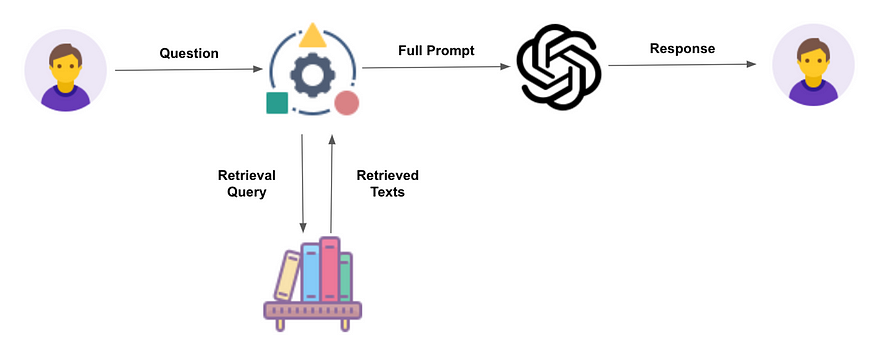
\includegraphics[width=0.8\textwidth]{images/rag.png}
    \caption{Esquema de funcionamiento de una arquitectura RAG.}
    \label{fig:rag}
\end{figure}
\subsection{Ontologías}
Una ontología en el campo de la informática es una especificación formal y explícita de una conceptualización. En otros términos, una ontología es una representación de un conjunto de conceptos dentro de un dominio y las relaciones entre esos conceptos. 

El lenguaje usado para definir ontologías es el \textit{Web Ontology Language} (OWL), que es un lenguaje de marcado semántico para publicar y compartir ontologías en la web. OWL es desarrollado por el \textit{World Wide Web Consortium} (W3C) y es una extensión de \textit{Resource Description Framework} (RDF), que es un modelo de datos basado en grafos para describir recursos web.

Como posible base de conocimiento relevante para la generación de consultas JQL se propone crear una ontología que represente las reglas que existen en las consultas JQL. La información que se pretende representar en la ontología se ha extraído directamente de la documentación oficial de Jira, brindada por Atlassian, donde se detallan las reglas que se deben seguir para la creación de consultas JQL \cite{jiradocs}. Esta ontología serviría para interpretar las reglas que hay que seguir al generar consultas JQL, además, consta de ejemplos en cada una de las clases definidas, que ayuda a comprender mejor el funcionamiento de las reglas.

Esta ontología ha sido desarrollada utilizando el software \textit{Protégé} \cite{protege}, una herramienta de código abierto para la creación de ontologías desarrollada por la Universidad de Stanford.
\section{Diseño}
En esta sección se describirá el punto de partida del asistente JiraGPT Next y el diseño que se ha propuesto como mejora para la precisión de las consultas generadas. Se presentarán 3 alternativas utilizando arquitecturas RAG, que buscan dotar al modelo de información sobre la generación de consultas JQL.

Para estas tres propuestas, se ha hecho un estudio del estado del arte y se han consultado varios artículos que tratan de realizar mejoras similares a las expuestas en este trabajo, logrando inspiración en ellos. Por lo que, se van a probar 3 bases de conocimiento distintas con las que aumentar el contexto que posee el modelo y buscar una mejora en la precisión de las respuestas. Se va a utilizar una ontología para representar las reglas del lenguaje de consulta JQL, una base de datos vectorial con embeddings de la documentación de JQL y un knowledge graph que contenga los datos de un proyecto de LKS Next-GobTech.

\begin{figure}[H]
    \centering
    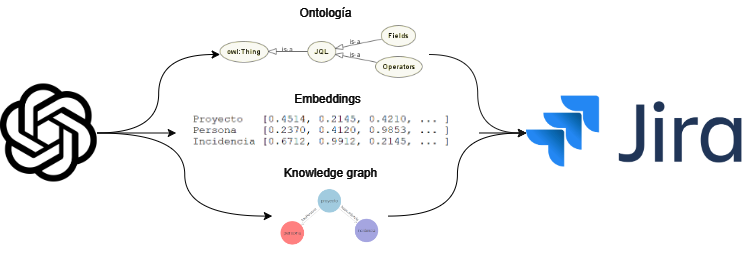
\includegraphics[width=0.95\textwidth]{images/diagrama_general.png}
    \caption{Diagrama de las tres propuestas, simbolizando las 3 bases de conocimiento distintas que van a ser estudiadas.}\label{fig:diagrama_general}
\end{figure}

\subsection{Estado inicial}
La aplicación desarrollada por Joel García y la presentada en este trabajo difieren en la manera de interactuar con el modelo. La aproximación que tomó Joel García fue la de realizar una ejecución de tres fases distintas, interactuando varias veces con el modelo. En el diagrama de la figura \ref{fig:diagrama_joel}, obtenido del trabajo de Joel García~\cite{jiragpt}, muestra el flujo de trabajo de la aplicación JiraGPT Next en su estado inicial.

\begin{figure}[H]
    \centering
    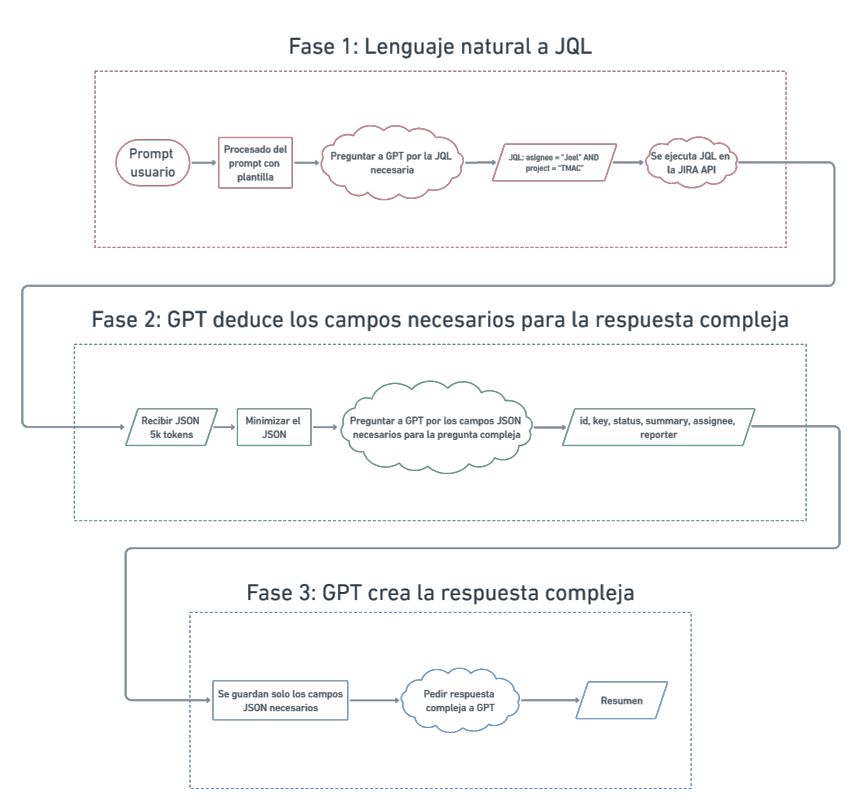
\includegraphics[width=0.95\textwidth]{images/diagrama_joel.png}
    \caption{Diagrama de las tres fases de la aplicación JiraGPT Next en su estado inicial~\cite{jiragpt}.}\label{fig:diagrama_joel}
\end{figure}

Durante la primera fase se preprocesaba la pregunta para adaptarla con plantillas y otorgar algo de contexto e indicaciones al modelo, se enviaba la pregunta y se postprocesaba la respuesta para limpiar cualquier tipo de comentario adicional que imposibilitase la ejecución de la consulta JQL. Durante esta misma fase se realizaba la llamada a la API de Jira con la consulta JQL generada ya procesada y se recogía el JSON devuelto.

La segunda fase consistía en limpiar el JSON para reducir campos de la respuesta que no contienen información relevante. En caso de no haber activado el botón de pregunta compleja, el resultado sería el JSON limpio, que se expone en la interfaz al usuario. En caso de haber activado la pregunta compleja, se haría una segunda llamada al modelo para que decidiese cuáles de los campos del JSON que se han conservado son relevantes para responder a la pregunta.

La tercera fase, que se ejecutaba independientemente de si la pregunta compleja ha sido activada, consistía en una tercera llamada para que realizase un resumen de lo preguntado. De esta manera, el usuario recibía tanto los campos que había solicitado como un resumen que respondiese a su pregunta de manera más directa.

Este proceso utilizaba la libería de Python que ofrece OpenAI para comunicarse con el modelo, de manera que resulta necesario adaptar el código para que funcione con esta librería. Lo que se propone desde este trabajo, también es una mejora en la interacción con el modelo, ya que se va a utilizar Langchain, una librería que permite la abstracción del uso del modelo, por lo que es más sencillo realizar llamadas a cualquier modelo de nuestra elección, sin tener que depender de las librerías de cada uno de los proveedores de estos modelos.

\subsubsection{Precisión inicial}
Para evaluar el estado inicial del modelo se ha de poner en contexto la técnica utilizada para evaluar la precisión: un \textit{benchmark} de 70 preguntas en el que se relaciona cada una con las incidencias que deberían ser recuperadas por el modelo.

La manera en la que se evalúa es ejecutando el conjunto entero de preguntas y comprobando si el asistente ha recuperado exactamente las incidencias contenidas en el conjunto de datos. Esto se decidió de esta manera ya que puede darse el caso en el que diferentes consultas devuelvan las mismas incidencias, lo que se consideraría correcto, con tal de que esas incidencias respondan a la pregunta del usuario.

En el momento de inicio de este trabajo, el asistente JiraGPT Next oscilaba entre un 45 y un 50\% de precisión en la recuperación de incidencias. Este resultado es fruto de una investigación sobre \textit{prompt engineering} realizada previamente por Joel García~\cite{jiragpt}. El objetivo, entonces, es buscar nuevas maneras de mejorar la precisión ofrecida por el modelo.
\subsection{Propuestas}
Se propone utilizar arquitecturas \aclink{RAG} para mejorar la precisión, ofreciendo al modelo información sobre la generación de consultas \aclink{JQL}. La idea detrás de esto es que, al tener un modelo de recuperación que pueda acceder a una base de conocimiento, el modelo de generación pueda generar respuestas más precisas y acordes al contexto proporcionado. Además, se propone un nuevo conjunto de datos:

Si bien el conjunto de datos inicial era robusto, se ha propuesto un nuevo conjunto, de 100 preguntas, que busca, no solo tener más datos, sino hacerlos más diversos y cambiar en cierto modo las preguntas para cubrir el máximo número de casos posible. Este conjunto de datos se ha pensado durante el desarrollo y las diferentes pruebas lanzadas y también se ha usado como apoyo un dataset existente en \textit{Hugging Face}~\cite{datasetHF}.

A continuación, se describirán las distintas alternativas propuestas para mejorar la precisión del modelo JiraGPT Next.

\subsubsection{Ontología}
Durante el inicio de este trabajo se consultaron artículos como \textit{Sequeda et al.}~\cite{sequeda2023benchmark}, que exploraban la posibilidad de utilizar ontologías en el prompt para mejorar la interpretación de los datos y la generación de consultas SQL, logrando resultados prometedores. Partiendo de esta idea, se propone entonces crear una ontología que represente las reglas que existen en las consultas JQL. La información que se pretende representar en la ontología se ha extraído directamente de la documentación oficial de Jira, brindada por Atlassian, donde se detallan las reglas que se deben seguir para la creación de consultas JQL \cite{jiradocs}. Esta ontología serviría para interpretar las reglas que hay que seguir al generar consultas JQL, además, consta de ejemplos en cada una de las clases definidas, que ayuda a comprender mejor el funcionamiento de las reglas.

Para crear esta ontología se ha utilizado el software \textit{Protégé}~\cite{protege}, una herramienta de código abierto para la creación de ontologías desarrollada por la Universidad de Stanford. La ontología se ha desarrollado siguiendo el estándar \textit{Web Ontology Language} (OWL), que es un lenguaje de marcado semántico para publicar y compartir ontologías en la web. OWL es desarrollado por el \textit{World Wide Web Consortium} (W3C) y es una extensión de \textit{Resource Description Framework} (RDF).

Durante esta parte, se considera una ejecución del benchmark como \textit{baseline} para comparar los resultados obtenidos con la ontología y sin ella. Esta primera ejecución se realizaría inyectando el archivo entero de la ontología en el prompt, de manera que el modelo pueda acceder a la información de la ontología y utilizarla para generar consultas más precisas.

Esta aproximación podría presentar resultados que, a priori, parecieran prometedores. Sin embargo, de cara al coste de inyectar un prompt tan grande, no es viable en un entorno de producción. Por ello, se propone una recuperación de información de la ontología dado un campo relevante para la pregunta del usuario. El diagrama en la siguiente figura muestra cómo será la interacción entre el modelo y la ontología.
\begin{figure}[H]
    \centering
    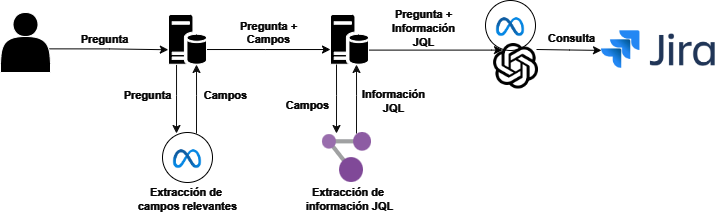
\includegraphics[width=0.95\textwidth]{images/rag_ontologia.png}
    \caption{Diagrama de RAG con ontología}\label{fig:ontologia}
\end{figure}
Si bien una ontología es una manera de representar un espacio de conocimiento, la documentación de Jira no presenta una estructura demasiado compleja que representar con la semántica de una ontología. Podría considerarse que, por ende, no es realmente necesario el uso de una ontología para representar las reglas de JQL. Sin embargo, tras lo realizado en este trabajo, no sería complicado utilizar otra ontología que reuniese información más compleja y permitiese explotar la semántica de la ontología para mejorar la generación de consultas JQL.

\subsubsection{Embeddings}
De igual manera que en el diseño de la ontología, se propone capturar en esta base de datos vectorial la documentación oficial de Jira. Esta base de conocimiento prueba a guardar los embeddings de los diferentes descripciones dentro de la documentación. La información que se ha considerado relevante ha sido cada campo/operador/función y sus respectivos ejemplos. De esta manera, dada una pregunta se podrían obtener los embeddings de las palabras y compararlas con los embeddings de la base de datos, de manera que el modelo obtenga ejemplos de campos relevantes para la pregunta del usuario.

Para capturar toda la información de la documentación se ha diseñado un programa en Python que realiza técnicas de \textit{web scraping} y recorre las entradas de la documentación extrayendo de las tablas los ejemplos. Una vez hecho esto, se guarda en un archivo de texto que será dividido en diferentes partes para ser procesado por el modelo de embeddings.
\section{Implementación}
A lo largo de esta sección se va a detallar la implementación de las distintas propuestas tecnológicas que se han descrito en el apartado anterior.

Para la implementación y el lanzamiento de muchas pruebas, se ha decidido ejecutar un LLM de manera local, ya que, de esta, manera, reducimos el coste de las llamadas a OpenAI a tan solo aquel que acarree el cálculo de los embeddings.

El modelo a utilizar será Llama3:8b, ejecutado en local mediante Ollama~\footnote{https://ollama.com} y al cual se harán llamadas a traves de programas Python, utilizando la librería Langchain~\footnote{https://www.langchain.com/}.

\subsection{Implementación de RAG: Embeddings}
Esta propuesta consta de una base de datos vectorial que contiene los embeddings de la documentación oficial de JIRA. Como software se ha optado por ChromaDB~\footnote{https://www.trychroma.com/} 0.5.0, una base de datos vectorial de código abierto que permite realizar búsquedas por similitud de vectores que, además, tiene una sencilla implementación con Langchain.

\subsubsection{Extracción de datos}
Para extraer los datos pertinentes de la documentación oficial de JIRA, se ha construido un \textit{web scraper} que recorre la documentación oficial de JIRA en el lenguaje Python que extrae de las tablas para cada entrada título, descripción y ejemplos. Estos datos se almacenan en un archivo de texto que posteriormente será dividido en diferentes partes para ser procesado por el modelo de embeddings.

Como modelo de embeddings se han utilizado los embeddings de OpenAI, que mediante una llamada con texto devuelven el vector a almacenar en la base de datos. Todo esto con un programa en Python que utiliza Langchain para abstraer el uso de ChromaDB y de la API de OpenAI.

\subsubsection{Interacción con el modelo}
Cuando una pregunta es recibida en el sistema, esta será procesada por los embeddings de OpenAI, lo que genera un vector que se compara con los vectores almacenados en la base de datos vectorial. Los vectores más cercanos a la pregunta serán devueltos, conteniendo la información de Jira pertinente. Esta información se inyecta en el prompt para que el modelo pueda generar una respuesta más precisa.
\subsection{Implementación de RAG: Ontología}
Como se ha mencionado en el apartado de diseño, se ha construido una ontología nueva utilizando la documentación oficial de JIRA para crear consultas JQL. Esta ontología describe los distintos tipos de operadores, campos y funciones que existen en este lenguaje de consulta. Además, se han añadido las relaciones entre estos elementos para que el modelo pueda inferir la información necesaria para responder a las preguntas. La idea detrás de esta ontología es modelar cómo funciona JQL, para que el modelo cometa menos errores de interpretación y pueda responder de manera más precisa. Se ha desarrollado tras el análisis de la documentación de JQL, siguiéndo prácticas para describir de manera correcta una ontología, respetando la semántica necesaria.

Esta ontología se ha desarrollado utilizando el software Protégé~\cite{protege}, gratuito y de código abierto, desarrollado por la universidad de Stanford. A través de la librería owlready2\footnote{\url{https://pypi.org/project/Owlready2/}} se ha podido cargar la ontología en Python y realizar consultas sobre ella. 

\subsubsection{Interacción con el modelo}
La manera más sencilla permitir al modelo interactuar con la ontología es inyectar el archivo entero en prompt, como describe Sequeda et al.~\cite{sequeda2023benchmark}. Sin embargo, esta aproximación no es viable en un entorno de producción, ya que inyectar un archivo tan grande en el prompt no es eficiente, pero se conserva de baseline, es decir, se van a realizar pruebas con esta aproximación para utilizar como resultado base y evaluar la extracción de información de la ontología. 

Para obtener información relevante de la ontología se ha utilizado un LLM que extrae los campos relevantes dada una pregunta, que son expuestos anteriormente en el prompt, ya que son campos descritos en la ontología que no conoce el modelo. La respuesta del modelo serán los 3 campos más relevantes de entre todos los descritos en el prompt y desde los que se realizará una consulta a la ontología para obtener la información relevante de la misma.

Esta información obtenida consistirá en los campos, operadores, ejemplos, descripción y subclases (de existir) que serán inyectados en el prompt para que el modelo pueda generar una respuesta partiendo de un mayor contexto.

Por ejemplo, para la pregunta `Dame las incidencias en progreso en el proyecto MFM` el modelo devolvería los campos `status` y `project` como los más relevantes, y, tras la consulta, tendríamos la siguiente información:

\begin{small}
\begin{verbatim}
['Status', ' Assignee']
Label: Status
Comment: None
Supports operators:
Subclasses of the field:
Abierto
Cerrado
En Progreso
Entregado
Reabierto
Resuelto
Validado


Label: Assignee
Comment: Search for issues that are assigned to a particular user. 
You can search by the user's full name, ID, or email address.
EXAMPLES:
Find issues that are assigned to John Smith:
assignee = "John Smith"or
assignee = jsmith
Find issues that are currently assigned, or were previously assigned, 
to John Smith:
assignee WAS jsmith
Find issues that are assigned by the user with email address 
bob@mycompany.com:
assignee = "bob@mycompany.com"
Supports operators: IS, WAS, !=, IS NOT, =, IN, CHANGED, NOT IN
Subclasses of the field:
\end{verbatim}
\end{small}

\newpage\printbibliography
\addcontentsline{toc}{section}{Referencias}
\end{document}
